\chapter{System design}
\label{hardware}

The system requirements are specified in the assignment instructions.


\section{Recommendations}\label{recommendations}

\begin{enumerate}
\item
  Independently fuse the buck converter and H-bridge. This allows a fuse
  to be removed to isolate part of the circuit when finding a fault,
  such as a short across the power rails.

\item
  Have a zener diode to protect against overvoltage when your group
  member inadvertently cranks up the voltage from the bench power
  supply.

\item
  Have current limiting resistors for all off-board signals.

\item
  Have plenty of testpoints, especially for power supplies and
  signals.  You will never have enough!

\item
  Have at least one grunty ground testpoint for attaching a scope ground
  clip.

\item
  Have a dedicated PIO pin to drive a testpoint that you can use to
  trigger an oscilloscope for debugging.

\item
  Have the SAM4S \pin{ERASE} pin connected to a test point close to a 3.3\,V
  testpoint. This is useful to completely erase the SAM4S flash memory
  when nothing works.

\item
  Have a MOSFET or servo interface for controlling something dastardly!

\end{enumerate}


\section{Standard chassis}

You can build your own racer or use the standard chassis.  The
standard chassis comes with:
%
\begin{itemize}
\item A pair of \href{https://www.pololu.com/product/3065}{6\,V DC
  motors} with a stall current of 1.5\,A at 6\,V.  They have a 100:1
  gearbox and a no-load speed of 330\,rpm at 6\,V.

\item A bumper with microswitch.

\item An on/off switch and fuse for the battery.

\item Battery and holder.
\end{itemize}
%
It is available from Diego in the Electronics Lab.  If you wish to
make your own chassis, Diego can supply the bumper, battery, and
motors.


\begin{figure}[!h]
  \centering 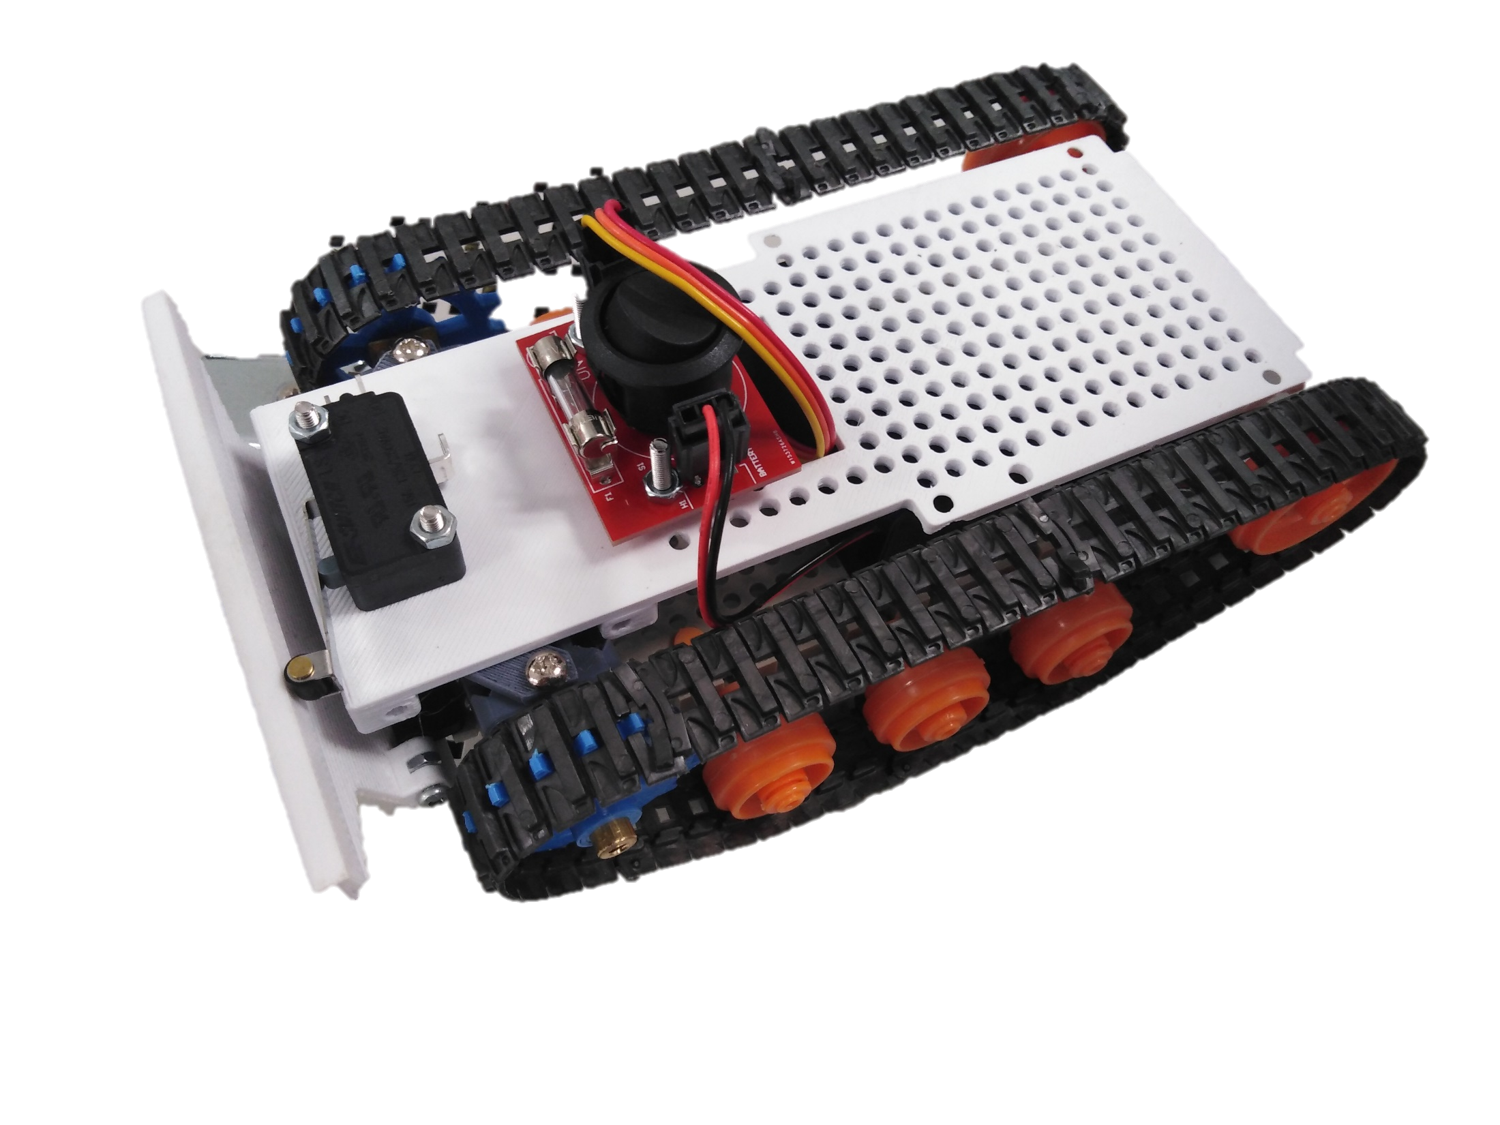
\includegraphics[width=5in]{figs/chassis.jpg}
  \caption{Photo of the standard chassis.}
  \label{fig:chassis}
\end{figure}



\section{SAM4S MCU}\label{sam4s-mcu}

The SAM4S MCU is overkill for this assignment but is typical of ARM
processors used for bare-metal applications.  The particular chip we
are using is the SAM4S8B.  This was made by Atmel and is now owned by
Microchip.  The datasheet is available
at \url{https://www.microchip.com/en-us/product/ATSAM4S8B}.

The SAM4S8B has a 32-bit ARM Cortex M4 RISC CPU that can run at
120\,MHz and has 512\,KB of flash memory and 128\,KB of SRAM.


\subsection{Power pins}\label{power-pins}

The SAM4S has four grounds. They \textbf{must} all be connected. There
are also seven power pins. These \textbf{must} all be connected since
they power different parts of the chip. Note, some pins require 3.3\,V
while others require 1.2\,V. The 1.2\,V is generated by an internal
voltage regulator.


\subsection{Peripheral pins}\label{peripheral-pins}

\textbf{Many of the peripheral pins are dedicated and cannot be
  reassigned in software}, e.g., SPI, TWI, and USB pins. Note, there
are restrictions on the PWM pins.  See Table~11-2 in the SAM4S
datasheet for the pin assignments.  Also see \hyperref[PIO pins]{PIO
  pins} for electrical characteristics.

By default the \pin{PB4} and \pin{PB5} pins are configured for the
JTAG debugger.  These can be used for general PIO after setting an
internal bit.  See \protect\hyperref[disabling-jtag-pins]{disabling
JTAG pins}.

The logic levels are set by the voltage on the VDDIO pin (usually
3.3\,V).  \pin{PA12}--\pin{PA14} and \pin{PA26}--\pin{PA31} can
sink/source 4\,mA.  The USB pins (\pin{PB10}--\pin{PB11}) can
sink/source 30\,mA.  The rest can only sink/source 2\,mA of current.

The pullup and pulldown resistors are typically 100\,k$\Omega$.  On
reset, pullup resistors are enabled.


\subsection{USART/UART}\label{usartuart}

The SAM4S has two USARTs and two UARTs. The USARTs can emulate a
UART, have hardware flow control, and have a better driver so they are
recommended if you need a UART interface.


\subsection{PWM}\label{pwm}

The SAM4S can generate four independent PWM signals. There are
restrictions on which SAM4S pins they come out on. Note, the PWMLx and
PWMHx signals are complementary (i.e., one is low while the other is
high).

\subsection{TWI}\label{twi}

The SAM4S has two TWI peripherals (that can act as a master and
a slave) with dedicated TWD and TWCK pins. External pull-up resistors
are required.  TWI1 shares pins with JTAG; you will need to disable
JTAG in software.

\subsection{SPI}\label{spi}

The SAM4S has a single SPI peripheral with dedicated SCK, MISO, and
MOSI pins. Any PIO pin can be used for the chip select\footnote{For
  high speed operation (not needed for this assignment), you should
  use one of the dedicated chip select pins.}.

\subsection{ADC}\label{adc}

The SAM4S has a single ADC with a multiplexer to select one of a
number of analogue inputs.  It can sample at 1\,MHz.

\subsection{USB}\label{usb}

The SAM4S has a single USB peripheral connected to the DDP and DDM
pins. 27 ohm series termination resistors are required, placed close to
the SAM4S.

\section{Other chips}\label{other-chips}

\subsection{DRV8833 dual H-bridge}\label{drv8833-dual-h-bridge}

The DRV8833's datasheet is available at
\url{https://www.ti.com/product/DRV8833}.

The H-bridge has four modes: forward, reverse, slow decay (brake), and
fast decay (coast).  With slow decay mode, the motor is shorted so
that it stops faster.  With fast decay mode, the motor is
open-circuited and so it takes longer to stop.  However, there is
little difference in practice, due to friction in the gearbox.

If you want control over fast decay and slow decay in both forward and
reverse you will need \textbf{four} independent PWM signals. The SAM4S
can provide four independent PWM signals but be \textbf{careful} since
PWMxH and PWMxL are complementary signals driven from the same PWM
source.

If you are clever, you can drive the H-bridge with only two PWM
channels.  If you are not so clever, you will have fast decay in one
direction and slow decay in the other.

The capacitor connected to the bootstrap pin must be rated for
16\,V. The datasheet recommends an X7R dielectric.

\subsection{NRF24L01+ radio}

\begin{figure}[!h]
  \centering 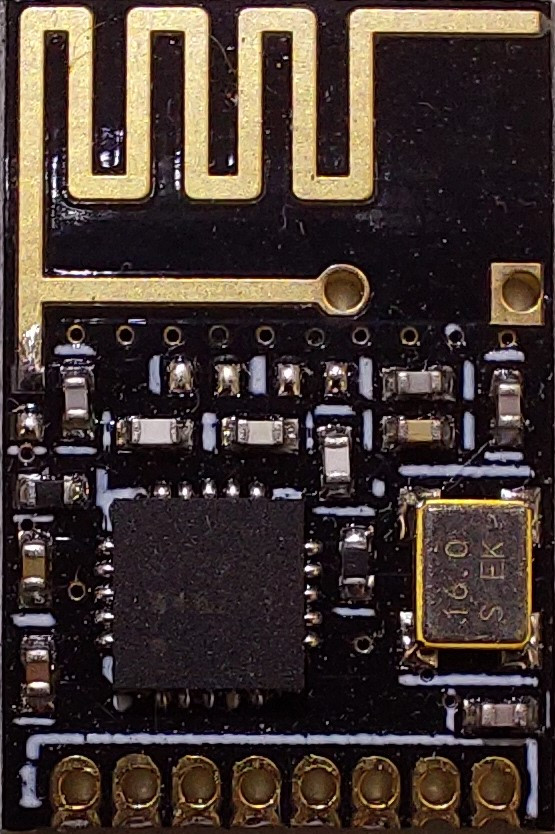
\includegraphics[width=1in]{figs/nrf24.jpg}
  \caption{Photo of NRF24 radio.}
  \label{fig:nrf24}
\end{figure}

The nRF24 module we provide is actually a tiny PCB with all of the high
frequency analogue components populated for you. This module breaks out
the SPI communication pins, the power supply pins, and two signal pins
that you will need to connect to your microcontroller. The CE and IRQ
pins can both go to general PIO pins while the SPI pins (MOSI, MISO,
SCLK, CSN) need to be connected to the SAM4S SPI peripheral. The
nRF24L01 datasheet and other documentation for the breakout board is
available at \url{https://www.sparkfun.com/products/691}.

As this radio is ultimately an analogue circuit and any noise on the
power supply can affect the signal quality, we recommend using a
separate 3V3 regulator and using a low pass filter to provide the best
power.  Instead of a resistor, a ferrite bead is better.

\begin{figure}[h]
  \centering
  \begin{circuitikz}
    \draw (-1, 0) node[left] {\SI{3.3}{\volt}} to[R=\SI{1}{\ohm}, o-] (2, 0)
    to[C=\SI{10}{\micro\farad}, *-*] (2, -2);

    \draw (-1, -2) node[left] {GND} to[short, o-] (2, -2);
    \draw (2, 0) to[short] (4, 0);
    \draw (2, -2) to[short] (4, -2);
    \draw (6, 0.5) -- (4, 0.5) -- (4, -2.5) -- (6, -2.5);
    \node[right=0.2] at (4, 0) {VDD};
    \node[right=0.2] at (4, -2) {GND};
    \node at (6, -1) {nRF24};
  \end{circuitikz}
  \caption{Power supply filtering; a ferrite bead is better than a resistor.}
  \label{fig:radio-filtering}
\end{figure}

You cannot have a PCB plane near the antenna of the radio otherwise
the \textbf{range will be severely limited}.

The radio operates around 2.4 GHz and has 128 programmable channels,
each of 1 MHz.  Note, some of these channels use the same spectrum as
Bluetooth and WiFi.  A 5 byte address is appended to the start of each
transmission and the receiver will only respond when the address
matches.

The radio interfaces to the SAM4S using the SPI bus. The IRQ
pin is driven low to indicate a packet has been received.



\subsection{MPU9250 IMU}\label{mpu9250-imu}

This contains a three axis accelerometer, a three axis gyroscope, and a
three axis magnetometer. It appears that the magnetometer has been
bolted on to the accelerometers/gyroscopes and requires more hoop
jumping in software to make it work. Documentation is available at
\url{https://invensense.tdk.com/products/motion-tracking/9-axis/mpu-9250/}.

It has two different I2C addresses (0x68 and Ox69) depending on the
state of the \pin{AD0} pin.


\subsection{Buck converter}\label{buck-converter}

The ADP2302ARDZ-5.0 buck converter is a switch-mode regulator that
converts the battery voltages to 5\,V DC.  It seems to operate with a
battery voltage as low as 5.4\,V.  This part has a fixed voltage
output and so a voltage divider is not required in the feedback
circuit.


\subsection{Voltage regulators}\label{voltage-regulators}

There are many flavours of \wikiref{voltage_regulators}{voltage regulator}.
Some are better for digital applications, some are better for analogue
applications, some are better for low power applications, etc.

If you are using a voltage regulator with an enable pin, do not forget
to allow for the time for the output voltage to ramp up. This can be
tens of milliseconds depending on the capacitive load and current draw.

Note, some regulators have pins that you must not connect. Some have
multiple pins for the same purpose; these must all be connected.


\subsection{Level-shifter}\label{level-shifter}

A level-shifter is required to convert the 3.3\,V signal levels from
the SAM4S to 5\,V for the \hyperref[LED-tape]{LED tape}.  This can be
achieved with a MOSFET and pullup resistor or with a dedicated
level-shifter chip.  Note, the SN74LVC1T45 level-shifter part in the
ENCE461 Altium library is bidirectional; you need to configure the
\pin{DIR} pin appropriately.



\section{External components}

\subsection{Battery}

The Wacky Racer batteries are Turnigy 5-cell 6\,V, 2300\,mAh, NiMH
with a three pin JST connector.  To preserve the battery life it is
imperative to not draw current when the battery voltage is below 5\,V.
Note, when fully charged, the battery voltage may be 7.5\,V.

The battery uses a standard RC servo connector: 3 pin 0.1'' (pin 1
GND, pin 2 5V, pin 3 NC). We suggest connecting both the first and
third pins to ground to allow the battery to be plugged in in both
orientations. The 461 Altium library has a component named
`Battery\_HEADER\_3pin' that is suitable to use.

\subsection{LED Tape}
\label{LED-tape}

The LED tape is a daisy-chained string of WS2812 smart LEDs.  These
LEDs use a clever mechanism to pass the RGB data down the
string\footnote{Each element consists of red, green, and blue LEDs
  with an 8-bit shift register to control the brightness for each
  colour.  These shift registers are chained together.} with different
pulse lengths for 1 and 0.  They are connected as shown in
\reffig{LED-chaining}.

\begin{figure}[h]
  \centering
  \begin{circuitikz}

    \draw (0, 0) node[left] {\SI{5}{\volt}} to[short, o-] (13, 0);
    \draw (0, -4) node[left] {GND} to[short, o-] (13, -4);

    \draw (1, -1) rectangle (4, -3);
    \draw (5, -1) rectangle (8, -3);
    \draw (9, -1) rectangle (12, -3);

    \draw (0, -2) node[left] {DIN} to[short, o-] (1, -2) node[right] {DIN};
    \draw (4, -2) node[left] {DO} -- (5, -2) node[right] {DIN};
    \draw (8, -2) node[left] {DO} -- (9, -2) node[right] {DIN};
    \draw (12, -2) node[left] {DO} -- (13, -2);

    \draw (2.5, 0) -- (2.5, -1) node[below] {VDD};
    \draw (6.5, 0) -- (6.5, -1) node[below] {VDD};
    \draw (10.5, 0) -- (10.5, -1) node[below] {VDD};

    \draw (2.5, -4) -- (2.5, -3) node[above] {GND};
    \draw (6.5, -4) -- (6.5, -3) node[above] {GND};
    \draw (10.5, -4) -- (10.5, -3) node[above] {GND};
  \end{circuitikz}
  \caption{Chaining of smart LEDs in the LED-tape.}
  \label{fig:LED-chaining}
\end{figure}

This means you will need to provide a three pin header (0.1" standard
header) with the pinout: pin 1 \SI{5}{\volt}, pin 2 signal, pin 3
ground. Each individual LED has a maximum supply current
of \SI{60}{\milli\ampere} (\SI{20}{\milli\ampere} per red, green, blue
channel). We will provide up to half a metre of LED tape to each car
or hat, giving a maximum number of 30 LEDs to be driven.

\begin{figure}[!h]
  \centering 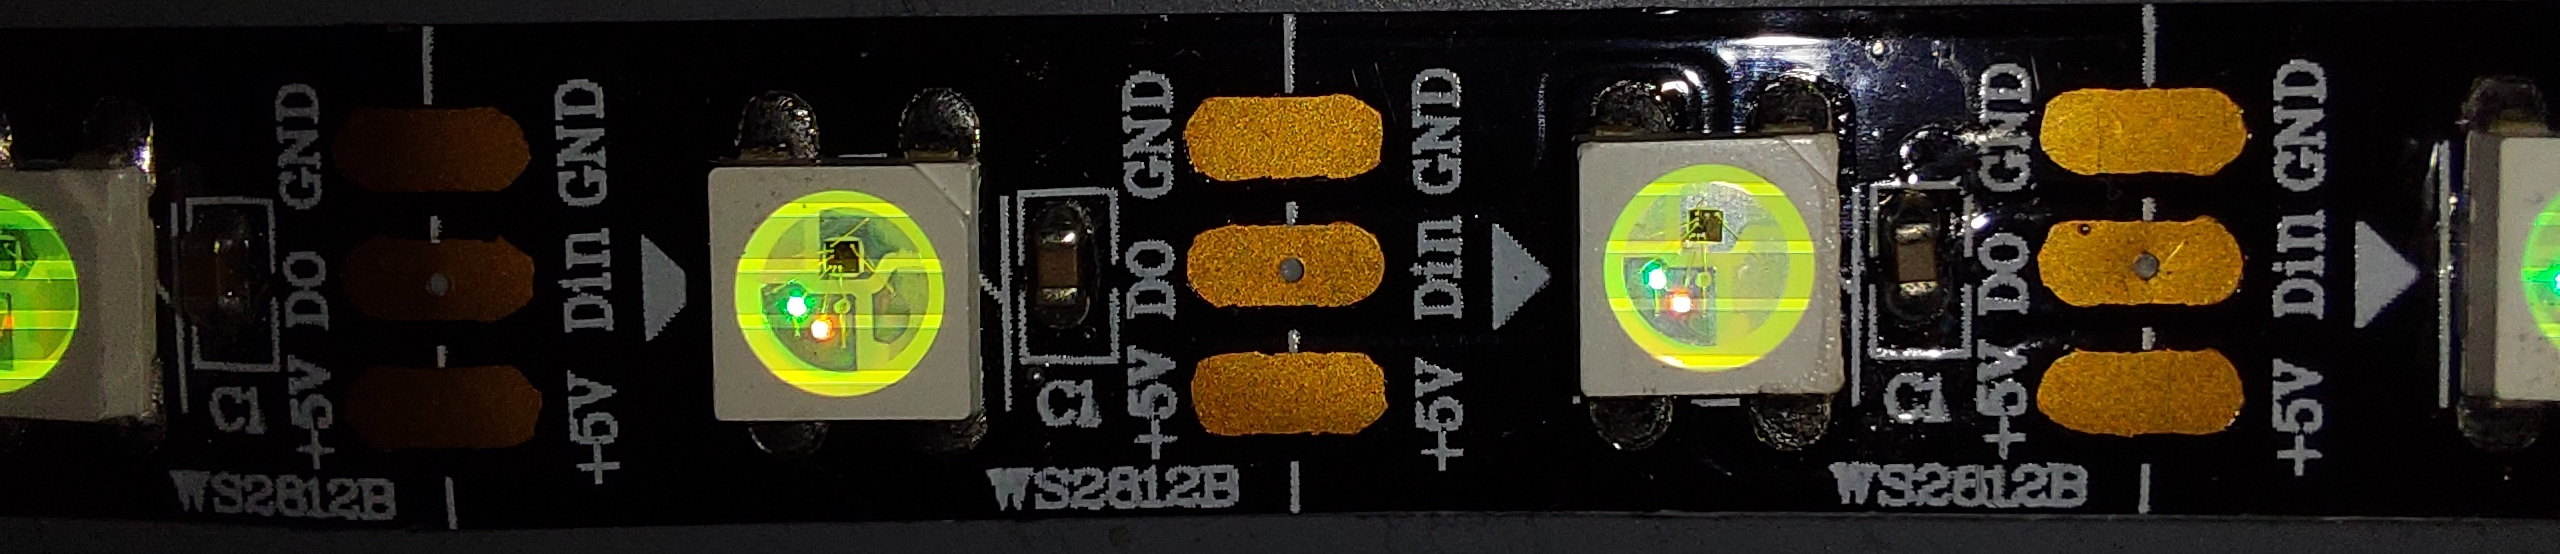
\includegraphics[width=6in]{figs/led_tape.jpg}
  \caption{Photo of a section of LED tape.}
  \label{fig:led-tape}
\end{figure}


\subsection{Bumper}

The provided bumper senses the contact through a simple limit switch. This
switch is normally open and on contact will close.

\begin{figure}[h]
  \centering
  \begin{circuitikz}

    \draw (0, 0) to[short, o-*] (2, 0) to[switch] (2, -2) node[ground]{};
    \draw (2, 0) to[R] (2, 2) node[vcc]{\SI{3.3}{\volt}};

    \draw[blue, dashed] (1.5, -0.5) rectangle (2.5, -1.5);
    \node[blue, right] at (2.5, -1) {limit switch};

  \end{circuitikz}
\end{figure}

Note that the pullup resistor shown could simply be the internal
pullup resistor on a PIO pin. The connector for the limit switch
should be a simple 2 pin 0.1" header.

\subsection{Buzzer}

The buzzers supplied are passive piezo-electric devices. Applying a
voltage across the two terminals causes the element to
deform. Applying an alternating current to the device generates an
audible tone. The larger the applied voltage differential, the louder
the tone becomes. There are plenty of example circuits for piezo
buzzers available online.  Note, you need to be able to charge and
discharge the capacitance of the pizeocrystal.

\subsection{Motors}

The motors available in the provided chassis are
\href{https://www.pololu.com/product/3065}{6\,V DC motors} with a
stall current of 1.5\,A at 6\,V.  They have a 100:1 gearbox and a
no-load speed of 330\,rpm at 6\,V.  You need to add connectors for the
motors, either 2 pin 0.1" headers or screw terminals are suggested.


\subsection{Connectors}

\begin{enumerate}
\item USB micro or mini connector for debugging
\item 3 pin 0.1'' for LED tape (pin 1 5\,V, pin 2 signal, pin 3 ground)
\item 2 pin 0.1'' for bumper (pin 1 switch, pin 2 ground)
\item 10 pin IDE for serial wire debug
\item 3 pin JR battery connector (pin 1 GND, pin 2 VBAT, pin 3 GND)
\item motor connectors (for Racer)
\item connectors for dastardly stuff
\end{enumerate}


\section{Other components}

\begin{enumerate}
\item We recommend that you use components in the ECE Altium library.
  These are stocked in the SMT lab.  For any other components you may
  require, see Scott Lloyd in the SMT lab.
\end{enumerate}


\section{Reading datasheets}

The manufacturer will tell you what they are proud of on the first
page.  They will omit details of poor aspects.

There is a knack in reading a large datasheet.  Here's what I do
first:

\begin{enumerate}
\item Look at the example circuits.

\item Read the absolute maximum ratings.

\item Read the pin definitions.
\end{enumerate}


% SAM4S hardware checklist
